\subsubsection{Phobia}

\paragraph{Outline}

Strat ME clone. Has +1 bonuses (situationally good, either for combos or for early income and forced lines). Center and West have very fast expansion if uncontested (center > west). East and Islands (and sometimes other areas) can provide safer income. Veto it, cast it into the fire, destroy it.
\url{https://www.youtube.com/watch?v=0PIzMSeFc0Y} 3x4, neutrals: 2/4, wastelands 6/10, base +5.

\paragraph{Map Dynamics}

\begin{figure}[H]
  \centering
  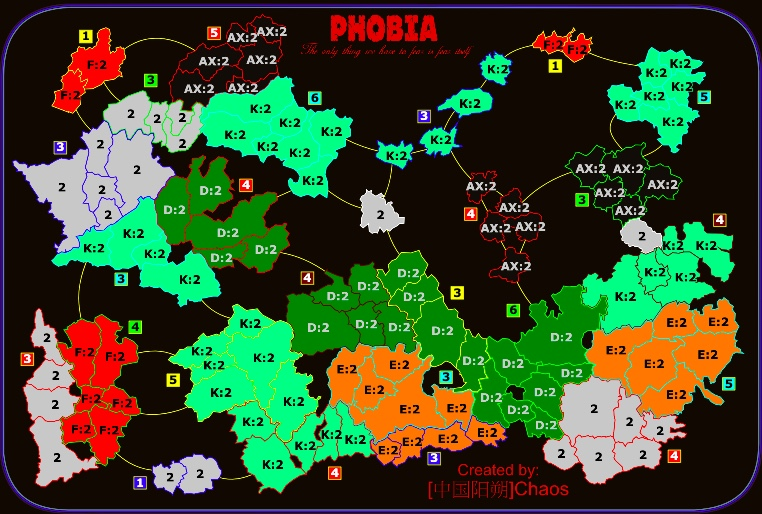
\includegraphics[width=0.8\textwidth]{Images/1800phobia.jpg}
  \caption{Bonus Win Rates for Games with Overall Winner Rating >=1800 in Phobia(n=421) (AX>D>K>Q>E>F>-).}
  \label{phobia_1800}
\end{figure}

\begin{itemize}
    \item AX >60\% Win Ratio
    \begin{enumerate}
        \item That +3 in the east has the highest WR but only 14 games in the database, among which games like \href{https://www.warzone.com/MultiPlayer?GameID=38294064}{this}, \href{https://www.warzone.com/MultiPlayer?GameID=33334645}{this} and \href{https://www.warzone.com/MultiPlayer?GameID=32179178}{this}. Very niche counter or combo to the red +4 or the light blue +5.
        \item The red +4 "Helminthophobia" runs this map (it is unbelievable to me this bonus is allowed to exist), it's an Indonesia on steroids. Picked in 232/421 games (most picked) and has >60 \% Win Ratio. Only single borders, really fast expansion in Blue +3, controls pathways to the west and center, just runs the map, more than even the south +2 does in Treasure Map.
        \item NW Red +5, "cynophobia", is just very strong in some distributions. Beneficial border against the +3, way too far away from everything else to counter it, and can combo three ways. a) with +3 for FTB or counter like \href{https://www.warzone.com/MultiPlayer?GameID=38753471}{here} b) with +6, c) with anything for the +5 bonus in 2 like \href{https://www.warzone.com/MultiPlayer?GameID=38047164}{here}
    \end{enumerate}
    \item D >55\% Win Ratio.
    \begin{enumerate}
        \item Uncontested triple +6 wins the game. But easy to cover and easy to spot if your opponent likes risky sets. The combo +4s in the center/west are very strong due to their proximity towards other income and how easy it is to defend against bonuses further away.
    \end{enumerate}

\end{itemize}


\paragraph{Picking Logic}

I generally find this boring the worse from the Strat ME clones due to how boring it can be on picks. In theory, it has less wastelands, more bonuses, an open map, but in reality, 8/10 distributions have +3 FTBs that run the map or +4 combos or even FTBs that also run the map. Props to that 1 in 20 games that has a triple +6 or a combo +5.
\\
\\
And the above isn't even the biggest issue, as in my opinion the +1s cost more than the variety they bring and the islands in the center/north are too strong. As in every WR template, position and army advantage matter a lot, the picks are kind of irrelevant in comparison to your moves as well as your leftovers. Pivoting and having armies in useful territories is equally important, as for example \href{https://www.warzone.com/MultiPlayer?GameID=39344277}{here} on Turn 15 I cannot afford to send my armies forward in risk of the blockade, and have to fight my way to eliminate Edge in the center with that stack or expand and pivot east to the Maroon +4.
\\
\\
The +1s are generally either of the following.
\begin{itemize}
    \item Positional picks like \href{https://www.warzone.com/MultiPlayer?GameID=36558136}{here by Octane}, slam a 1st pick there and hope for the best.
    \item Setup picks like \href{https://www.warzone.com/MultiPlayer?GameID=40571550}{here by Rufus}. Setup up the 5->10 income by end of Turn 2 to all in north. Good leftovers -> Win, Bad leftovers -> Loss. 
    \item \href{https://www.warzone.com/MultiPlayer?GameID=36549357}{Combo +5} in the NE.
    \item And then some niche games like \href{https://www.warzone.com/MultiPlayer?GameID=25558453}{here} setting up 11 in 2 and \href{https://www.warzone.com/MultiPlayer?GameID=41473762}{here} setting up 12 in 2. Overall, same idea as always. Small bonuses -> Fight early. Big bonuses -> Fight later.
\end{itemize}
You can get some ideas from the following games and different scenarios as in:
\begin{itemize}
    \item Contested FTB and combo +5, example \href{https://www.warzone.com/MultiPlayer?GameID=38753471}{here}, just 345 west FTB/combo and pray to jesus for good WR rolls
    \item triple +6 and combo +5 \href{https://www.warzone.com/MultiPlayer?GameID=33947836}{here}
    \item Scattered picks for later contact \href{https://www.warzone.com/MultiPlayer?GameID=33377309}{here}, \href{https://www.warzone.com/MultiPlayer?GameID=38375555}{here}
\end{itemize}
As well as a lot of ideas from clan league and nation's cup  2023 (\href{https://docs.google.com/spreadsheets/d/1QPKGgwToBd2prap8u3XVUx9F47SuvMH9wJruvG0t2D4/edit?usp=sharing}{Round 1})templates, since this is quite popular amongst a group of players I dare say don't really understand. WR in my opinion excels at templates that favor army maneuvers and this map is just void of enthusiasm, not a lot of spice or uniqueness. A lot of games will come down to your leftovers and if you are able to finish a 2nd bonus with 3 attacks on turn 3 or turn 4. For example \href{https://www.warzone.com/MultiPlayer?GameID=34443262}{here}, Octane's entire strategy on picks is to hit with stack the Brown +4 on Turn 3 if lucky, or on Turn 4 if not, after the FTB player expands there. The outcome is already predetermined, the players are wasting their time, and who will win after picks is entirely dependent on the luck on leftovers and RMO.  
\\
\\
\begin{figure}[H]
  \centering
  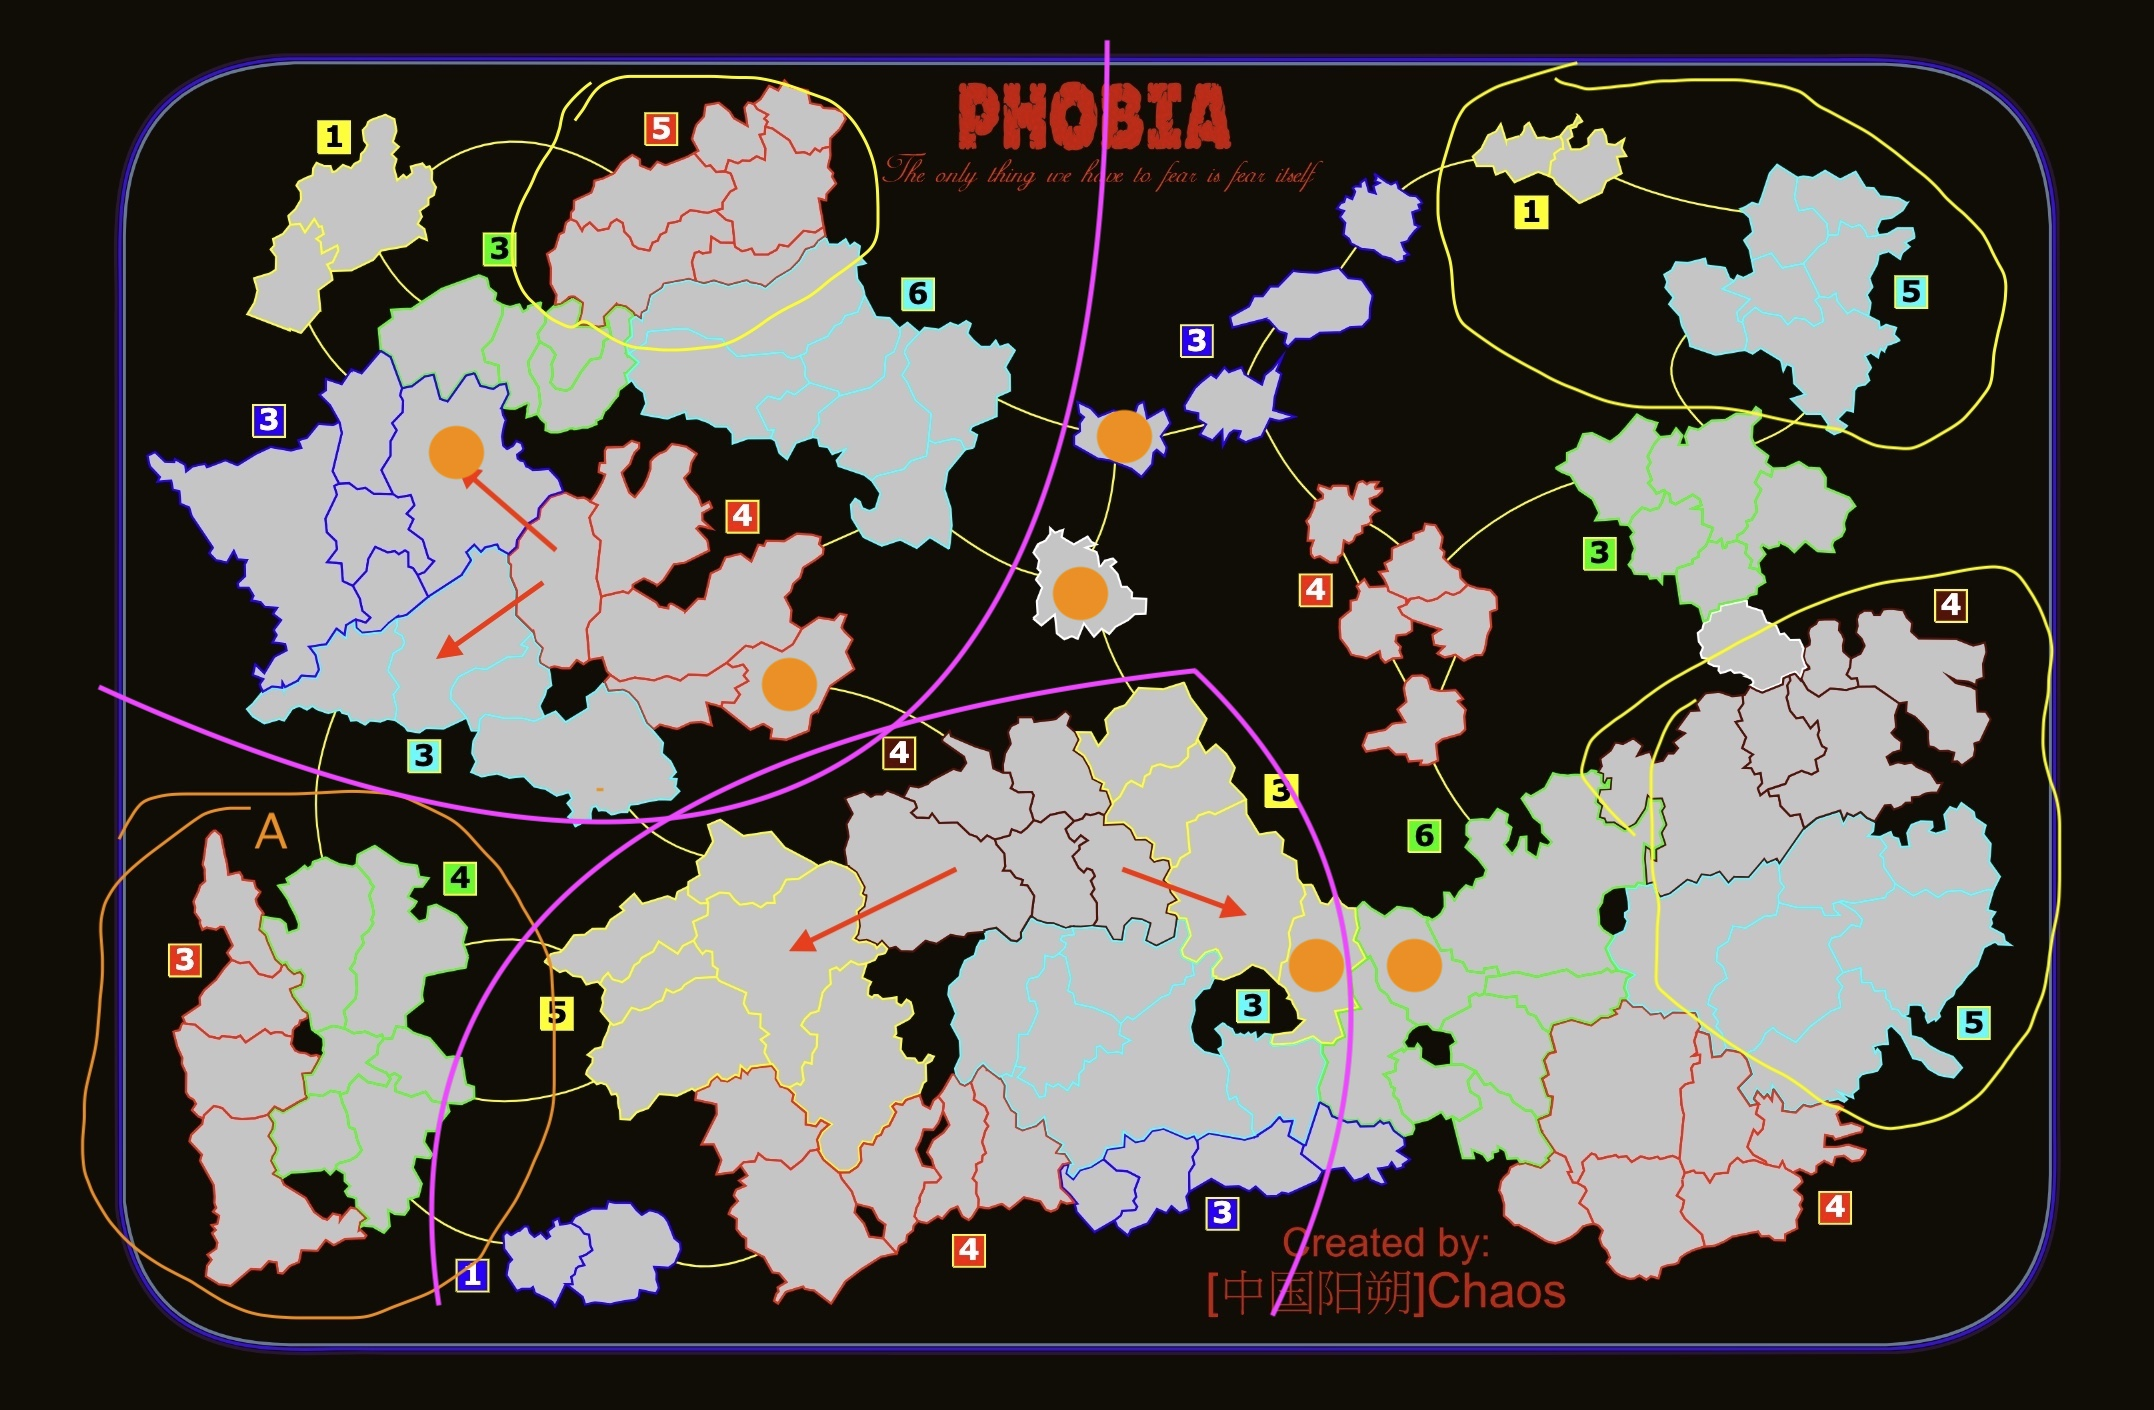
\includegraphics[width=0.7\textwidth]{Images/phobia zones.jpg}
  \caption{Phobia Zones}
  \label{phobia_zones}
\end{figure}

If you want to make decent picks in half a second, you can run the simple algorithm below. If yes, then do that step, if no proceed to next step.
\begin{itemize}
    \item Is there a +4 FTB in the center? Go or cover it.
    \item Is there an uncontested safe green +6 triple? Go or cover it.
    \item Separate the board into income zones that I direly need to cover. Figure \ref{phobia_zones} for reference.
    \begin{itemize}
        \item Zone A west is 99/100 times not even worth consideration. Yellow zones are for safe income or safe combos. Besides that, there's the turbo-broken island +4 and +3 region, the center and the red +4/light green +3 west. If you envision all these, you can sort of see 3-5 zones, that differ from board to board. Talking about:
        \begin{itemize}
            \item North West (can be 2 zones itself if it's red +4/light blue +3 vs red +5)
            \item Center
            \item Islands
            \item East, which has bigger and safer bonuses
        \end{itemize}
        \item Assess really fast do I need to cover all regions, yes or no. For example, \href{https://www.warzone.com/MultiPlayer?GameID=39333446}{here} the center is not worth your time and the islands + east counter each other. Conclude within 2 seconds that the easiest way to pick is 1/2 or 1/3 east or islands and 4 picks west for coverage or 1/2 east, 3 a safe income pick somewhere and 456 west.
        \item If you can't simplify the board as above, aim for bonuses that can provide you coverage, that are flexible. That's where the template becomes repetitive.
        \begin{itemize}
            \item The islands will give you a path to cover any region you won't get coverage in, but they might fall in income.
            \item The west red +4 "Selacophobia" is extremely underrated as it actually doesn't have double borders whatsoever. You can't solo pick it against the light blue +3 FTB or if it's contested from other sides but bare in mind how hard it is to break. Below it, the brown +4 in the center has the fastest expansion in the whole template. For example take a look in \href{https://www.warzone.com/MultiPlayer?GameID=35123636}{this game} around T4-T5 onwards (ignore how blind both were to the neutral between them, best example i could find), where if you give a couple of turns of tempo to the center player (Timi) as the remote safe income player (Mr.Carpenter), you just lose the game because the center will double it's income and hold the chokepoints.
        \end{itemize}
    \end{itemize}
\end{itemize}